% MIT License

% Copyright (c) 2022 Chiyuru

% Permission is hereby granted, free of charge, to any person obtaining a copy of this software and associated documentation files (the "Software"), 
% to deal in the Software without restriction, including without limitation the rights
% to use, copy, modify, merge, publish, distribute, sublicense, and/or sell
% copies of the Software, and to permit persons to whom the Software is
% furnished to do so, subject to the following conditions:

% The above copyright notice and this permission notice shall be included in all copies or substantial portions of the Software.

% THE SOFTWARE IS PROVIDED "AS IS", WITHOUT WARRANTY OF ANY KIND, EXPRESS OR IMPLIED, INCLUDING BUT NOT LIMITED TO THE WARRANTIES OF MERCHANTABILITY,
% FITNESS FOR A PARTICULAR PURPOSE AND NONINFRINGEMENT. IN NO EVENT SHALL THE AUTHORS OR COPYRIGHT HOLDERS BE LIABLE FOR ANY CLAIM, DAMAGES OR OTHER
% LIABILITY, WHETHER IN AN ACTION OF CONTRACT, TORT OR OTHERWISE, ARISING FROM,
% OUT OF OR IN CONNECTION WITH THE SOFTWARE OR THE USE OR OTHER DEALINGS IN THE SOFTWARE.

%%%%%%%%%%%%%%%%%%%%%%%%%%%%%%%%%%%%%%%
% 由驰雨的模板改编,版权见上
% 专供清华大学科学与工程计算课程上机报告使用
% Author: Polly Joe, Tsinghua University
%%%%%%%%%%%%%%%%%%%%%%%%%%%%%%%%%%%%%%%



% 此处是导言区,除了添加宏包不要改动
\documentclass[UTF8,twoside,zihao=-4,AutoFakeBold,scheme=chinese,openany]{ctexart}
\usepackage{tabto}
\usepackage{indentfirst}
\usepackage{longtable}
\usepackage{array}
\usepackage{float}
\usepackage{multicol}
\usepackage{multirow}
\usepackage{amsmath}
\usepackage{amsfonts}
\usepackage{cases}
\usepackage{cite}
\usepackage{geometry}
\usepackage{booktabs}
\usepackage{graphicx}
\usepackage{float} %设置图片浮动位置的宏包
\usepackage{subfigure} %插入多图时用子图显示的宏包
\geometry{a4paper,left=2cm,right=2cm,top=2cm,bottom=2cm}


\pagestyle{plain}
\CTEXsetup[format={\kaishu\bfseries}]{section} %设置章标题字号为Large,居左
\CTEXsetup[number={\chinese{section}、}]{section} %section形式改为一,二,三,..



\title{\textbf{\Large\kaishu 数值分析第一次上机练习报告\\ \large\kaishu ——线性方程组解法}}

\author{\normalsize\kaishu Polly Joe}
\date{}

\begin{document}
\maketitle


%%%%%%%%%%
% 问题描述
%%%%%%%%%%
\section{问题的描述}
设$H_n=[h_{ij}] \in \mathbb{R}^{n \times n}$是Hilbert矩阵,即
$$h_{ij}=\frac{1}{i+j-1}$$
对n=10,11,...,15恒成立。\\
(a) 取$x=
        \begin{pmatrix}
         1  \\
         ...\\
         1
    \end{pmatrix}\in \mathbb{R}^{n}$,令$b_n=H_nx$.再用Gauss消去法和Cholesky分解方法来求解$H_ny=b_n$,看看误差有多大.\\
(b) 使用正则化方法改善(a)中的结果.\\
(c) 用共轭梯度法和GMRES方法求解$H_ny=b_n$,并于前面的直接方法作比较.





%%%%%%%%%%%%%%%%%%%%%%%%%%%%%%%%%%%%%
% 方法描述
% 子标题可以按照自己喜好调整
%%%%%%%%%%%%%%%%%%%%%%%%%%%%%%%%%%%%%
\section{方法描述}
(a) \textbf{Gauss消元法和Cholesky分解法}

\setlength{\parindent}{2em}段落演示,每个段落都仿照这样就可以实现开头缩进两行。注意每次分段落的时候记得空行,否则不会缩进而是连在一起。

\setlength{\parindent}{2em}段落演示,每个段落都仿照这样就可以实现开头缩进两行。注意每次分段落的时候记得加上双斜杠或者空行,否则不会缩进而是连在一起。\\



(b)\textbf{Tikhonov正则化}

\setlength{\parindent}{2em}段落演示,每个段落都仿照这样就可以实现开头缩进两行。注意每次分段落的时候记得加上双斜杠或者多空一行,否则不会缩进而是连在一起。

\setlength{\parindent}{2em}段落演示,每个段落都仿照这样就可以实现开头缩进两行。注意每次分段落的时候记得加上双斜杠或者多空一行,否则不会缩进而是连在一起。\\

(c) \textbf{共轭梯度法和GMRES法}

\setlength{\parindent}{2em}段落演示,每个段落都仿照这样就可以实现开头缩进两行。注意每次分段落的时候记得加上双斜杠或者多空一行,否则不会缩进而是连在一起。

\setlength{\parindent}{2em}段落演示,每个段落都仿照这样就可以实现开头缩进两行。注意每次分段落的时候记得加上双斜杠或者空行,否则不会缩进而是连在一起。\\


%%%%%%%%%%%%%%%%%%%%%%%%%%%%%%%%%%%%%%
% 方案设计
%%%%%%%%%%%%%%%%%%%%%%%%%%%%%%%%%%%%%%

\section{方案设计}
\setlength{\parindent}{2em}我们通过编写MATLAB程序来进行线性方程组的求解。  


\section{计算结果及其分析}

\setlength{\parindent}{2em}图\ref{result}是我们根据程序计算结果得到的数据。

(a) \textbf{使用Gauss消去法和Cholesky分解的求解结果}

\setlength{\parindent}{2em}计算结果如图\ref{result}所示表格的第1-5列所示。

(b) \textbf{使用正则化改善后的求解结果}

\setlength{\parindent}{2em}计算结果如图\ref{result}所示表格的第6-9列所示。

(c) \textbf{使用共轭梯度法和GMRES法的求解结果} 

\setlength{\parindent}{2em}计算结果如图\ref{result}所示表格的第10-13列所示。\\


%%%%%%%%%%%%%%%%%%%%%%%%%%%%%%%%%%%%%%%%%%%%%%%%%%%%%%%%%%%%%%%%%%%%%%
% 插入表格和图片
% 此处为了方便,表格也使用图片(表格排版有Longtable无法处理合并单元格跨页的问题)
% 因为表格通常很长,可以分开截图
% 同时为保证清晰度,如果使用Excel建议导成pdf,再剪切生成png
% 如果使用这部分代码插入图片,请不要改动图片的尺寸,这是按照A4纸,页边距2cm设计的,目的是让表格单独占据一页,避免影响其他文本的排版
%%%%%%%%%%%%%%%%%%%%%%%%%%%%%%%%%%%%%%%%%%%%%%%%%%%%%%%%%%%%%%%%%%%%%%
\begin{figure}
\centering %表示居中
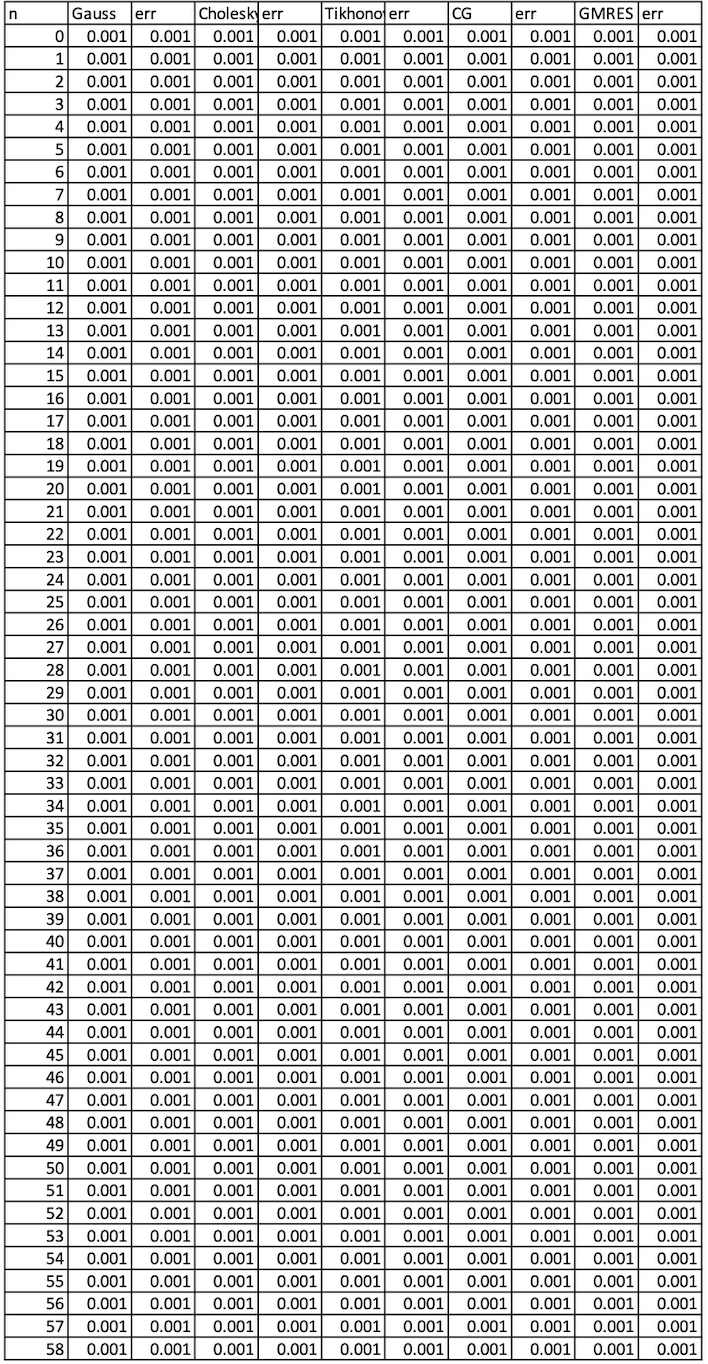
\includegraphics[width=17cm,height=24.7cm]{gauss.png}
\caption{计算结果}
%图片的名称
\label{result}
%图片的标签,用于文章中的引用,注意到标签的数字与实际文章显示的数字可能不同
\end{figure}





\section{结论}
\setlength{\parindent}{2em}段落演示,每个段落都仿照这样就可以实现开头缩进两行。注意每次分段落的时候记得加上双斜杠或者空行,否则不会缩进而是连在一起。


\end{document}
